\chapter{Approach}\label{chap:Approach}

\section{Main Objective}

In this thesis, we address a novel method to visualize multiple sequence alignments using colors. The main objective is to highlight sequence similarity (or alignment confidence) with color similarity.

In the alignment matrix, a well-aligned area should be represented by a solid-color shape, while a poorly-aligned one should become a mosaic of different colors. All the alignment-level information, such as evolutionary relationships, phylogenetic characteristics and alignment accuracy, should be revealed by the color pattern of the graph. Figure \ref{fig:app-wa} compares these two types of MSA regions and their coloring results.

\begin{figure}[hbt]
\centering
\subfloat[A well-aligned MSA region.]{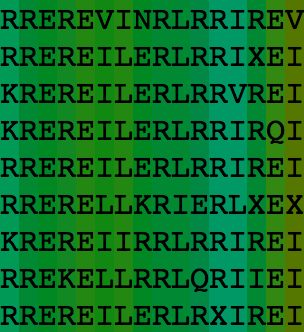
\includegraphics[width=0.35\textwidth]{figures/app-wa.png}}
\hspace{5mm}
\subfloat[A poorly-aligned MSA region.]{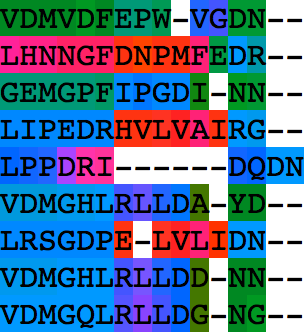
\includegraphics[width=0.35\textwidth]{figures/app-pa.png}}
\caption[Highlighting Sequence Similarity With Color Similarity]{Highlighting sequence similarity with color similarity.}\label{fig:app-wa}
\end{figure}

\section{Data Input}

Figure \ref{fig:app-wa}(a) shows a well-aligned MSA region, which contains many different types of amino acids. In order to demonstrate the good alignment quality, however, these amino acids are supposed to be painted with the same or similar colors. Obviously, the color assignment could not depend only on their residue types.

Therefore, unlike most traditional coloring approaches, we use an set of residue-residue similarity scores instead. Within each column of an MSA, all sequence residues are considered to be aligned together at the same equivalent position. We employ a third-party tool to examine each pair of these residues, and estimate the confidence that they should be aligned together. This confidence estimation can also be interpreted as a similarity score between the two residues.

Every pair of residues within a same column has a similarity score. These scores are used to determine how similar the residue colors should appear to each other. In a good-quality MSA region, all residues are confidently aligned together, therefore the colors would be same or similar. While in a bad-quality region, many alignments are doubtable, resulting in many different colors.

One widely used tool to generate this similarity score data set is GUIDANCE \cite{Penn:2010aa,Penn:2010ab}, which is designed for quantifying alignment uncertainty. GUIDANCE produces a confidence score in range of $[0, 1]$, named GUIDANCE score, for each symbol, symbol pair, column and sequence in the alignment. We take the symbol-pair GUIDANCE confidence scores as the input to Mavis.

\section{Color Generating}

The colors of the symbols are generated in such way that the color similarity represents the residue's alignment confidence. We have three steps to accomplish this goal.

\begin{figure}[hbt]
\center{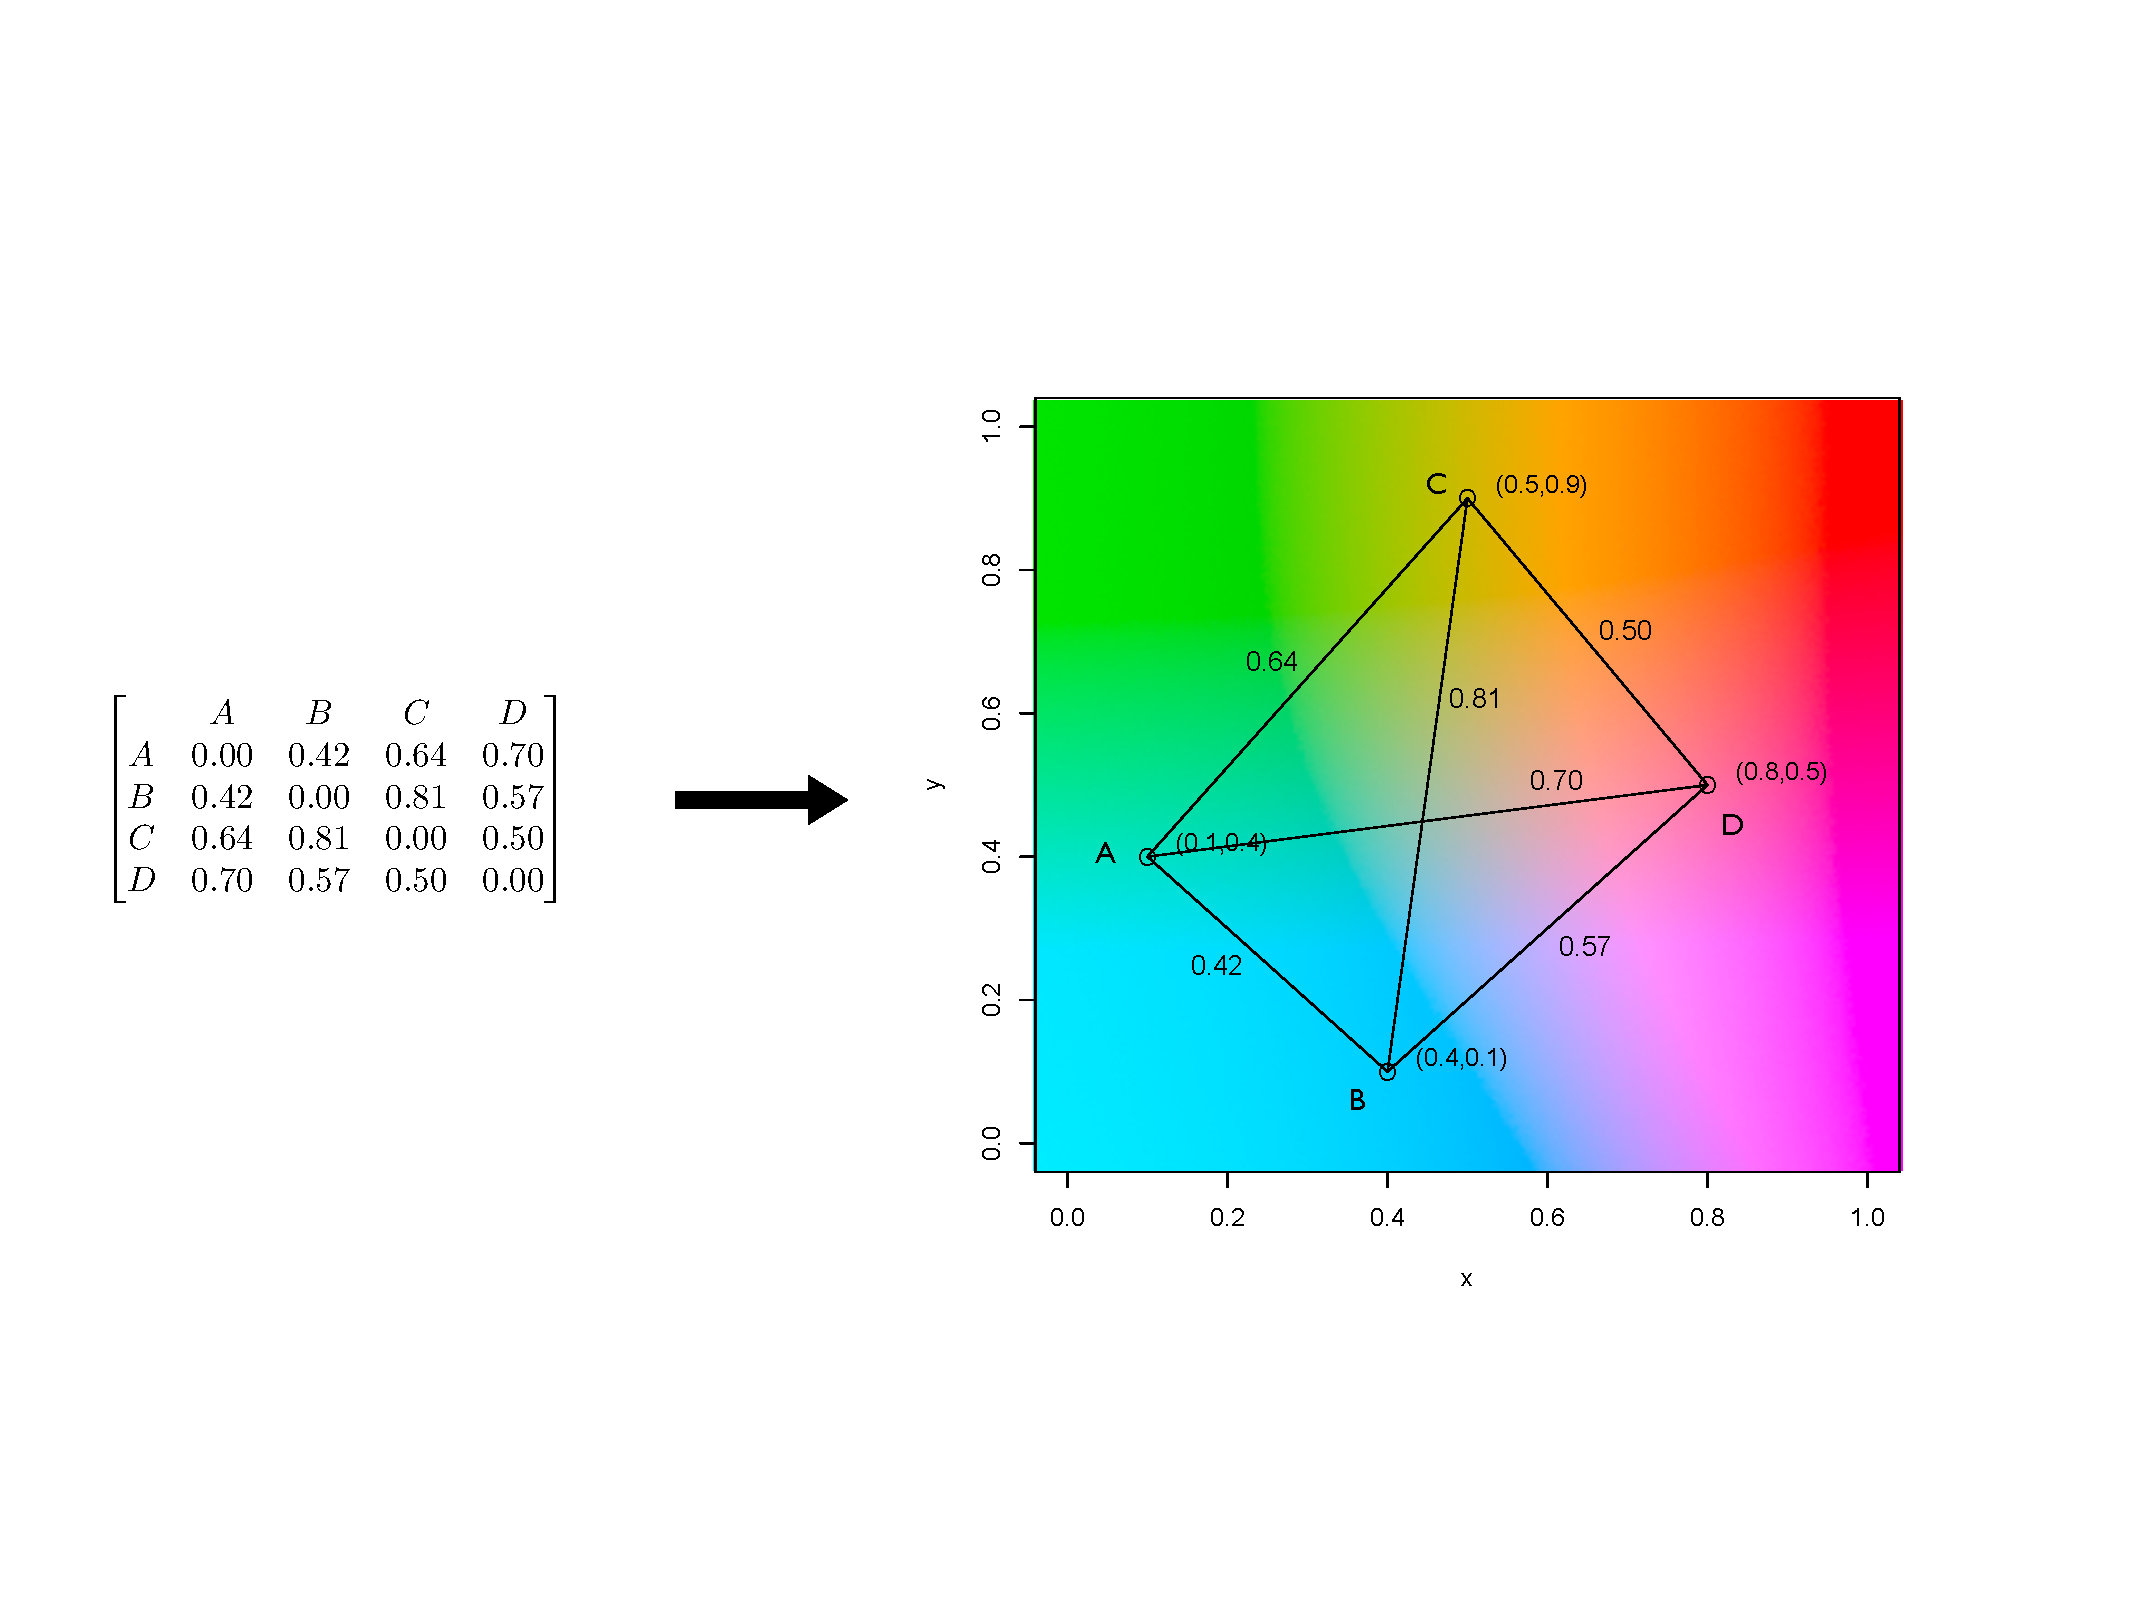
\includegraphics[width=\textwidth]{figures/chap2_color.pdf}}
\caption[Conversion from Distance Matrix into Colors]{A distance matrix is converted into points on a two-dimensional color space. The distances between points are approximately preserved. The color where a point is located is assigned to the corresponding alignment residue.}\label{fig:chap2_color}
\end{figure}

First, the confidence or similarity score is converted into a distance or dissimilarity score. From all these distances, an $N \times N$ distance matrix is constructed for each column, where $N$ is the number of residues in the same column. Second, from the distance matrix, the $N$ residues are mapped as $N$ points in a space of $N-1$ dimensions, such that for each pair of points, their Euclidean distance is equal to the value in the distance matrix. This mapping process is done by using a statistical technique called \emph{classical multidimensional scaling} \cite{Borg:1997aa}. Third, we map this space onto a color space, to find a color for each point. In an appropriate color space, the Euclidean distance approximately represents the color difference perceived by humans, so that our alignment confidence is linked with color similarity.

One problem appeared in the last step is that most color spaces are three-dimensional. In order to map the original space to a color space, it is necessary to reduce the dimension from $N-1$ to no more than 3, while the distances are still preserved as much as possible. Fortunately, classical multidimensional scaling is designed in such a way that the result has the largest possible variance on the first axis, the second largest on the second axis, and so on. Thus, we can reduce the space dimension by picking the first a few axes, and mostly preserve the distances.

\section{Color Optimization}

Up to now, our approach only operates on the column level and does not consider the relationship between columns. The only way to create a solid-color well-aligned region is to take cross-column information into account. Since there is no confidence score for two residues from different columns, the color difference between them does not mean anything, and should be eliminated as much as we can. In other words, the color graph needs to be as smooth as possible in the horizontal direction.

\begin{figure}[hbt]
\center{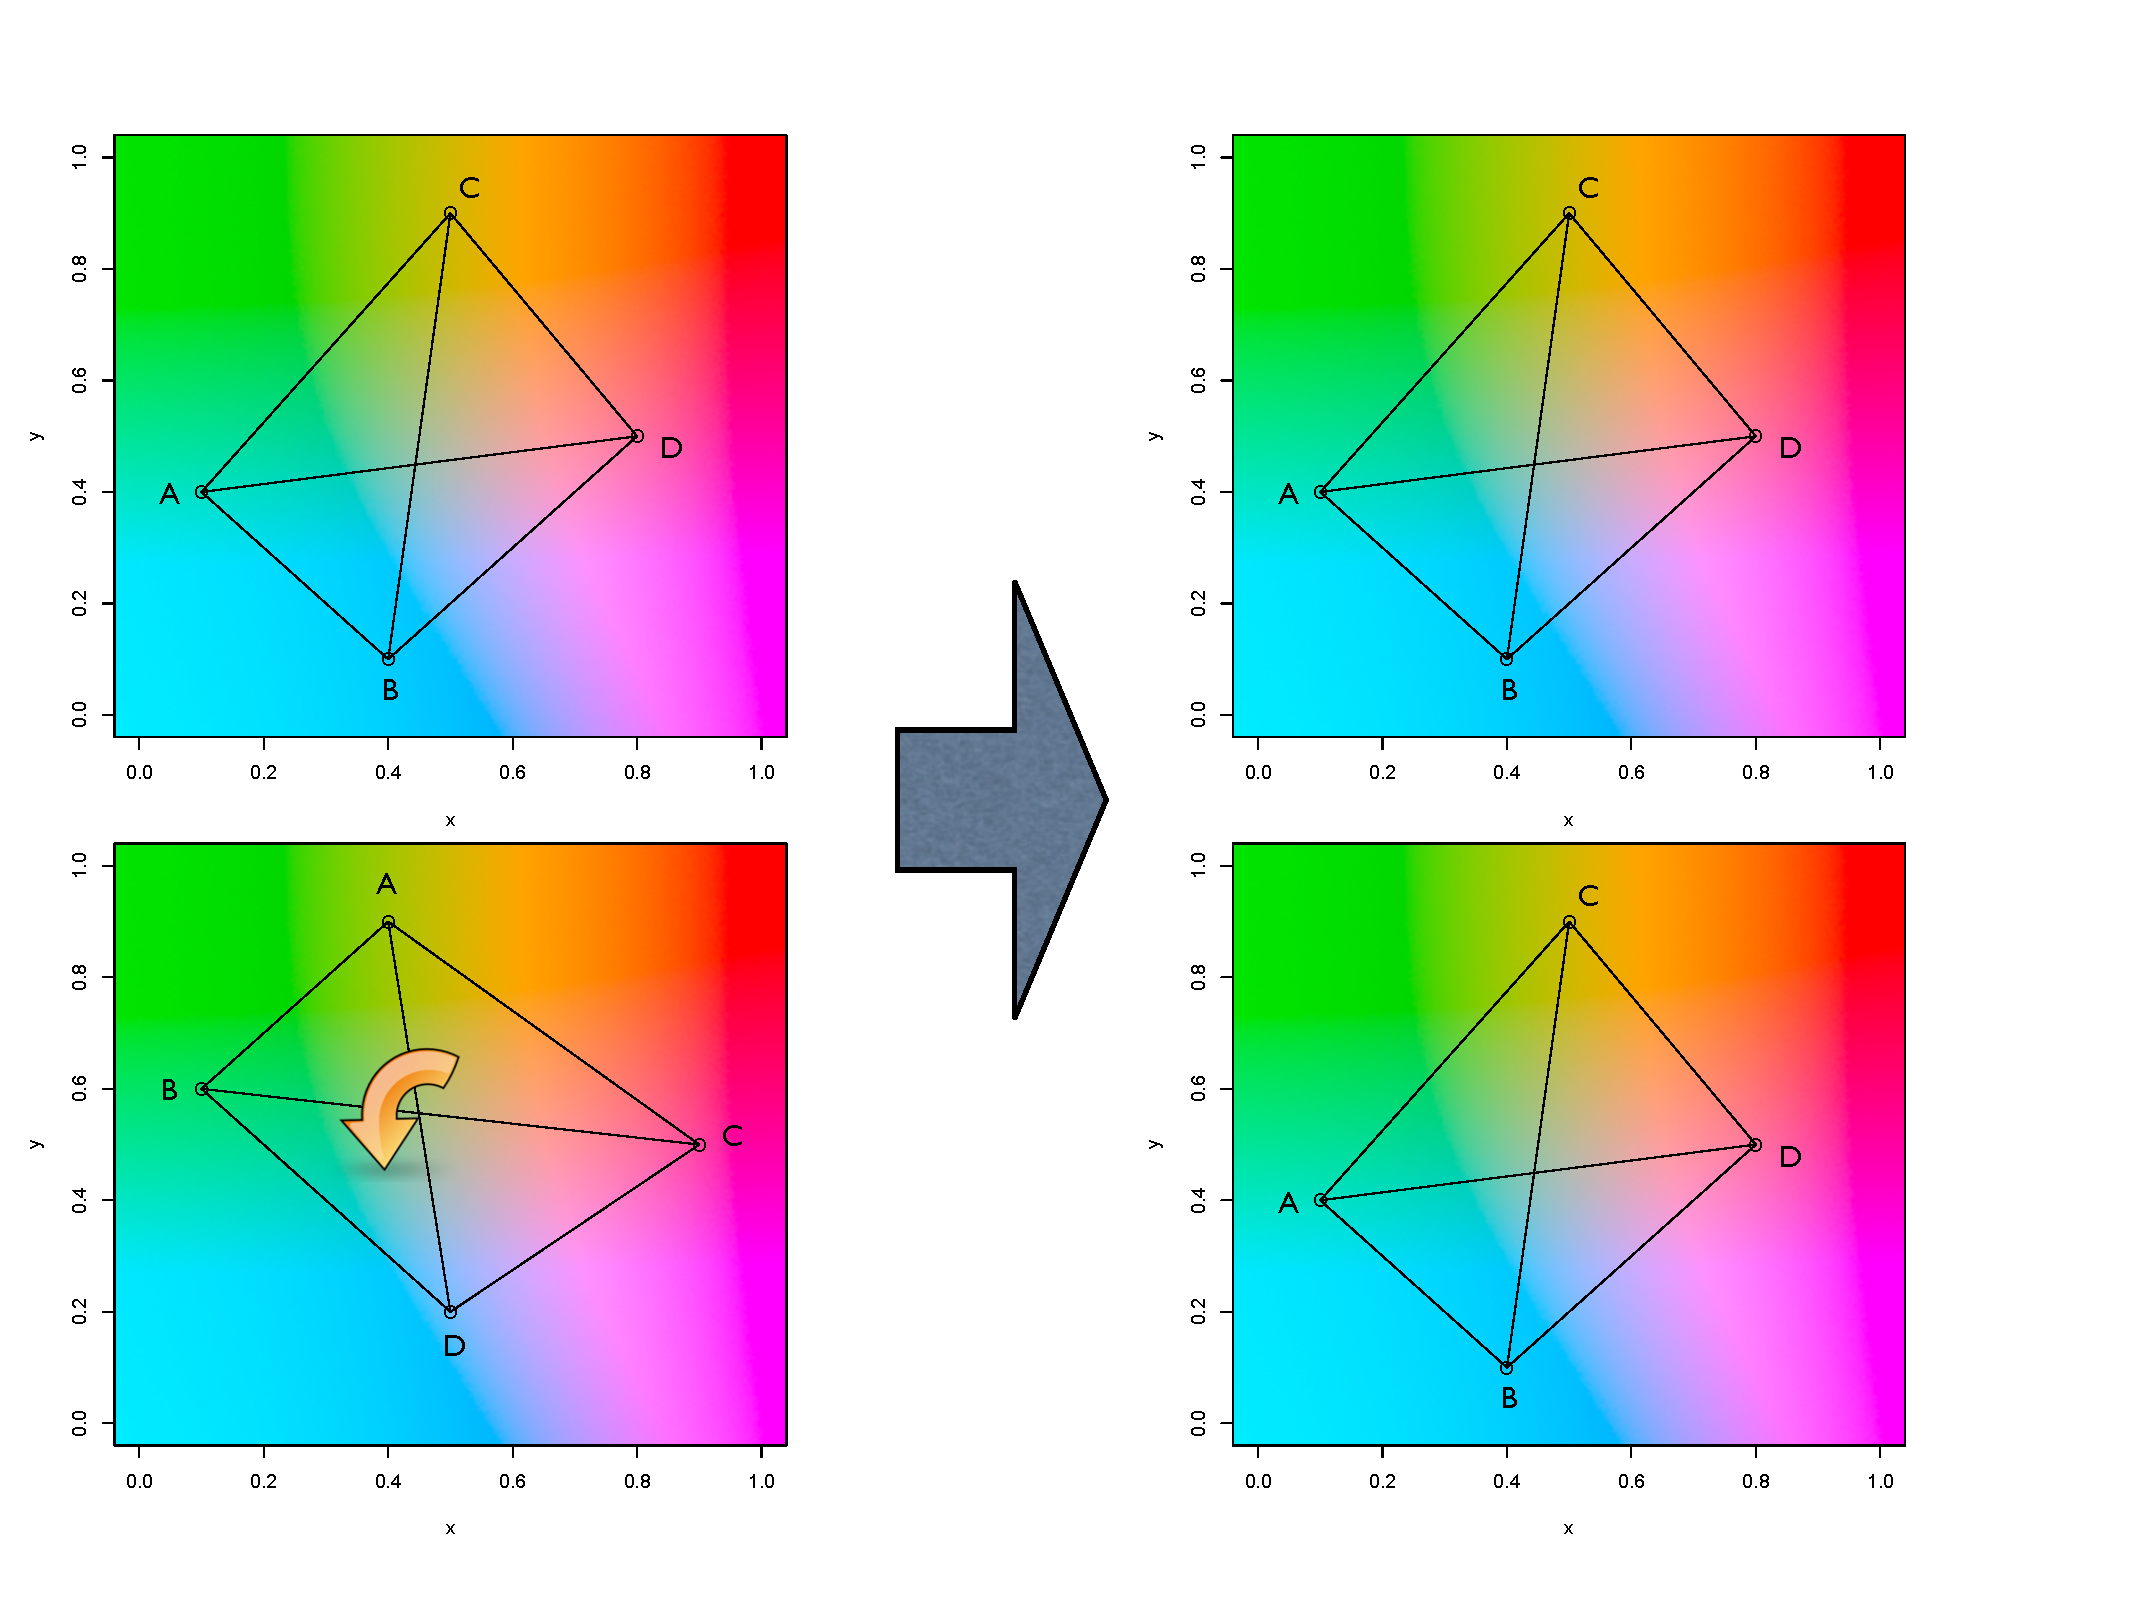
\includegraphics[width=\textwidth]{figures/chap2_rotate.pdf}}
\caption[Color Optimization by Rotation]{An example of color optimization by rotating.}\label{fig:chap2_rotate}
\end{figure}

A favorable feature of classical multidimensional scaling is the invariance under flips and rotations. All the points in the color space can be arbitrarily rotated and/or flipped, without changing the distance between any pair of symbols within a column. For instance, all reds and all greens are virtually identical in the sense of distances and quality of alignment. Converting them into the same color pattern will better support this idea and remove unnecessary color noises.

\begin{figure}[hbt]
\center{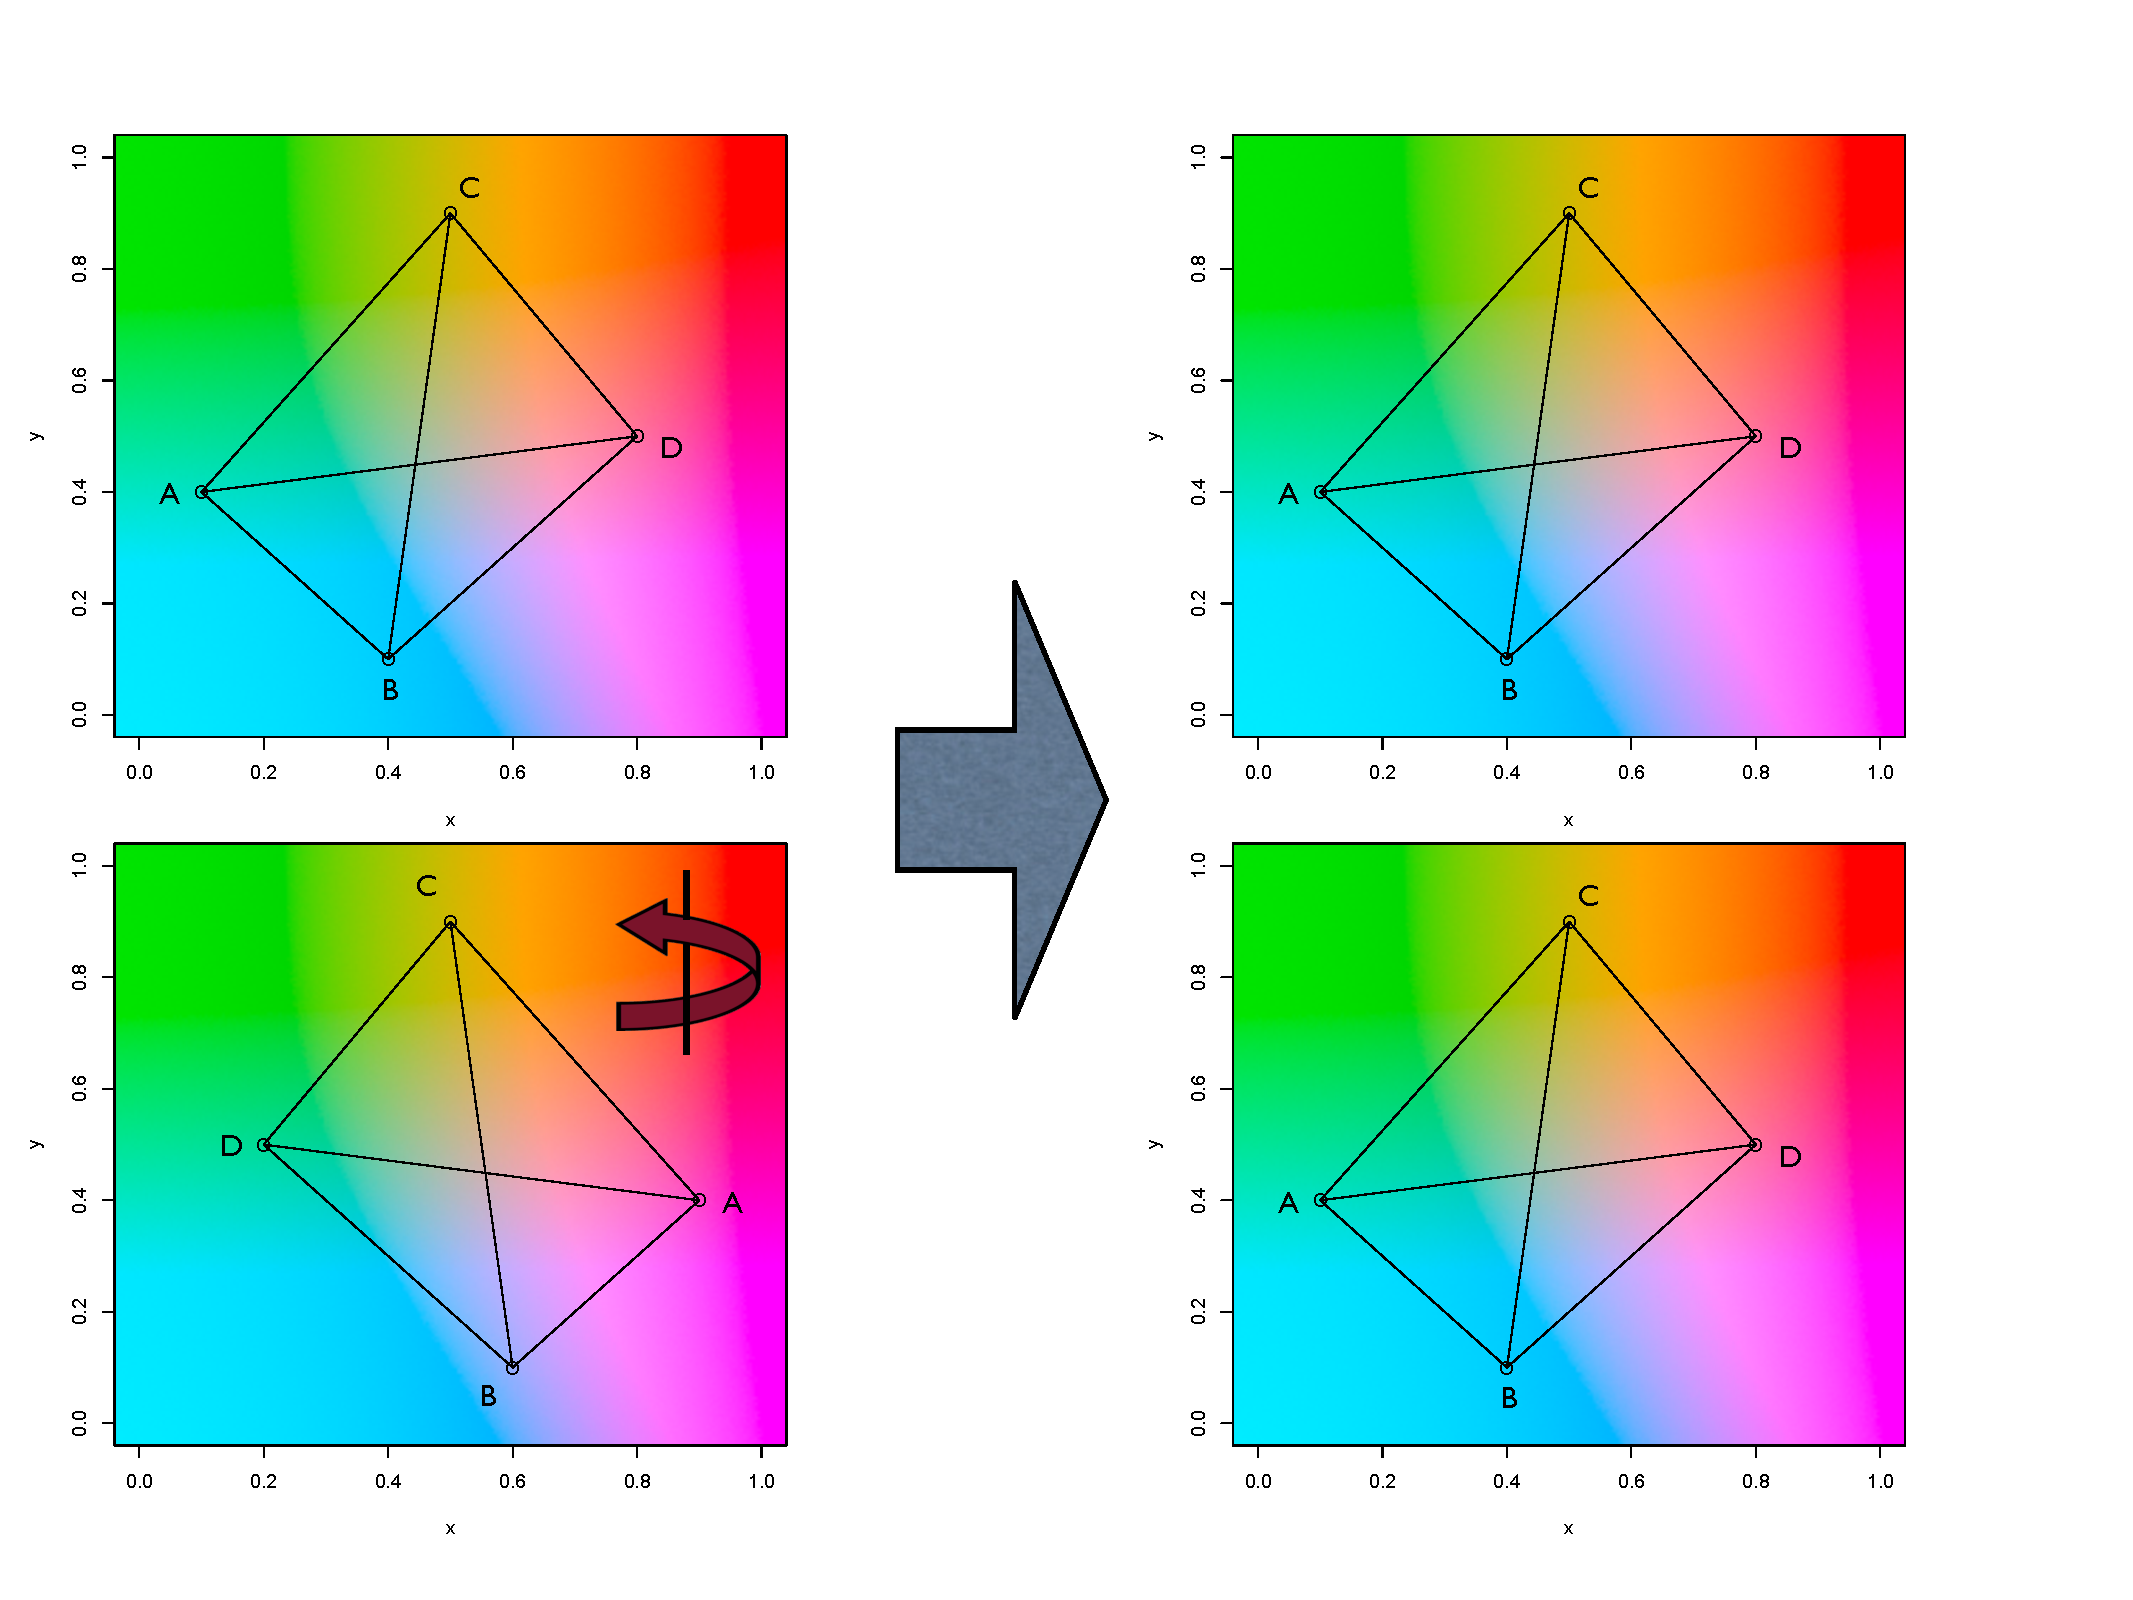
\includegraphics[width=\textwidth]{figures/chap2_flip.pdf}}
\caption[Color Optimization by Flipping]{An example of color optimization by flipping.}\label{fig:chap2_flip}
\end{figure}

To optimize our color assignment, we define a penalty function to quantify the overall color noise level of an alignment. This function calculates the color variance within each row and sum them up. By rotating and flipping, the ideal color assignment should result in the lowest penalty value.

For larger MSAs, finding the exact optimum may become time-consuming and sometimes impractical. Sub-optimal results are also acceptable for visualization purpose. In Mavis, we use an approximate solution to speed up the optimization procedure.

\section{MSA Visualization}

Mavis creates a colored matrix for an MSA. Users may choose to display residue symbols or not. The user interface is available in a web browser, in order to achieve better flexibility and portability. An API between the front-end and the back-end is designed to make the system extensible.

Figure \ref{fig:chap2_msa} shows an example of MSA matrix colored by Mavis.

\begin{landscape}
\begin{figure}[hbt]
\center{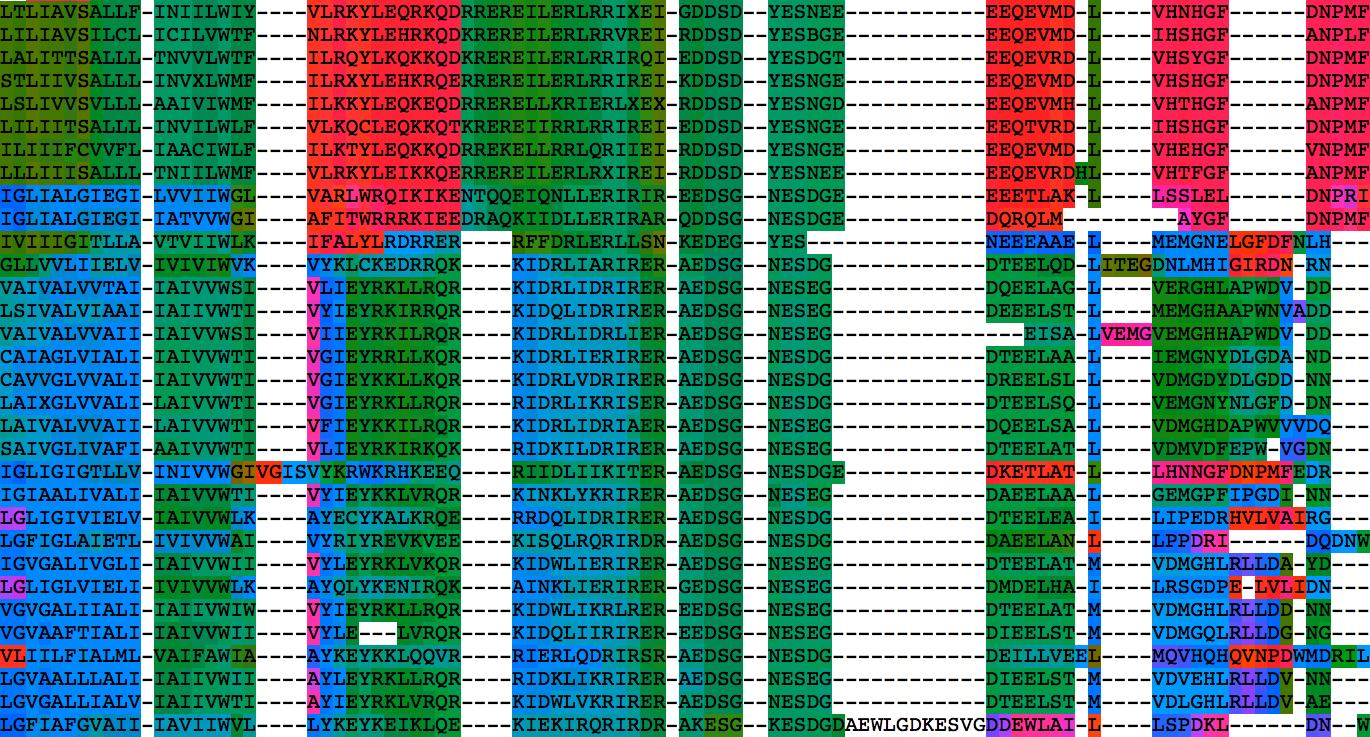
\includegraphics[height=0.73\textwidth]{figures/chap2_msa.png}}
\caption[Example of Mavis MSA Coloring]{An example of MSA matrix colored by Mavis.}\label{fig:chap2_msa}
\end{figure}
\end{landscape}
